\section{System Level Test}

Từ đoạn code mẫu \ref{pseudo-code:Serial} được nêu trong bài báo, có vài điểm cần phải phải tối ưu trong quá trình có thể chuyển từ giải thuật của bài báo xuông được phần cứng.

\subsection{Xây dựng Bộ tính giá trị trung bình của mảng}

\begin{lstlisting}[style=StyleCode, language=C, caption={Tính giá trị Trung bình.}]
	SIZE_TYPE_T C_Framework_RTL::P_Cal_Mean(std::vector<SIZE_ARR_T> &arr, IndexType si, IndexType ei){
		SIZE_TYPE_T t_sum = 0;
		for(int i =si; i <= ei; i++){
			t_sum += arr[i];
		}
		SIZE_TYPE_T t_div = 1;
		t_div = t_sum / (SIZE_TYPE_T)(ei - si + 1);
		return t_div;
	}
\end{lstlisting}

Với một bộ tính giá trị trung bình bằng cách đọc tất cả các giá trị trong mảng để tính được giá trị tổng quát của mảng. Còn giá trị số lượng phần tử được tính bằng công thức \texttt{(SIZE\_TYPE\_T)(ei - si + 1)} để chuyển từ giá trị HEX qua Float. Kết hợp thêm bộ kiểm tra các trường hợp đặc biệt của vùng dữ liệu:

%\begin{lstlisting}[style=StyleCode, language=C, caption={Tính giá trị Trung bình và Tìm trường hợp đặc biệt.}]
%	status_rtl_e C_Framework_RTL::P_SS_Check(std::vector<SIZE_ARR_T> &arr, IndexType si, IndexType ei, SIZE_TYPE_T &mean){
%		bool is_Similar     = true;
%		bool is_Acsending   = true;
%		bool is_Decsending  = true;
%		SIZE_TYPE_T temp_sum = 0;
%		for(int i = si + 1; i <= ei; ++i){
%			temp_sum += arr[i - 1];
%			if(arr[i] != arr[i - 1]){
%				is_Similar      = false;
%			}
%			if(arr[i] < arr[i - 1]){
%				is_Acsending    = false;
%			}
%			if(arr[i] > arr[i - 1]){
%				is_Decsending   = false;
%			}
%		}
%		temp_sum += arr[ei];
%		mean = temp_sum / (SIZE_TYPE_T)(ei - si + 1);
%		if(is_Similar){
%			return RTL_SIMILAR;
%		}
%		else if(is_Acsending){
%			return RTL_ACSENDING;
%		}
%		else if(is_Decsending){
%			return RTL_DESCENDING;
%		}
%		else{
%			return RTL_NORMAL;
%		}
%	};
%\end{lstlisting}
\begin{lstlisting}[style=StyleCode, language=C, caption={Tính giá trị Trung bình và Tìm trường hợp đặc biệt.}]
	status_rtl_e C_Framework_RTL::P_SS_Check(std::vector<SIZE_ARR_T> &arr, IndexType si, IndexType ei, SIZE_TYPE_T &mean){
		bool is_Similar     = true;
		bool is_Acsending   = true;
		bool is_Decsending  = true;
		SIZE_TYPE_T temp_sum = 0;
		for(int i = si; i < ei; ++i){
			temp_sum += arr[i];
			if(arr[i] != arr[i + 1]){
				is_Similar      = false;
			}
			if(arr[i] > arr[i + 1]){
				is_Acsending    = false;
			}
			if(arr[i] < arr[i + 1]){
				is_Decsending   = false;
			}
		}
		temp_sum += arr[ei];
		mean = temp_sum / (SIZE_TYPE_T)(ei - si + 1);
		if(is_Similar){
			return RTL_SIMILAR;
		}
		else if(is_Acsending){
			return RTL_ACSENDING;
		}
		else if(is_Decsending){
			return RTL_DESCENDING;
		}
		else{
			return RTL_NORMAL;
		}
	};
\end{lstlisting}

\subsection{Xây dựng bộ thực hiện phân hoạch mảng theo giá trị trung bình}

\begin{lstlisting}[style=StyleCode, language=C, caption={Phân hoạch dữ liệu theo giá trị trung bình.}]
	IndexType C_Framework_RTL::P_Partition_Iterative(std::vector<SIZE_ARR_T>& arr, IndexType si, IndexType ei, SIZE_TYPE_T mean_value) {
		IndexType pi = si;
		SIZE_ARR_T temp_a = 0;
		SIZE_ARR_T temp_pi = 0;
		for (IndexType i = si; i <= ei; ++i) {
			temp_a = arr[i];
			temp_pi = arr[pi];
			if (temp_a < mean_value) {
				arr[i] = temp_pi;
				arr[pi] = temp_a;
				pi++;
			}
		}
		return (pi > si) ? (pi - 1) : si; 
	}
\end{lstlisting}

Với việc tiến hành đọc dữ liệu trước khi so sánh dữ liệu với \texttt{pivot} giúp ta tối ưu và làm rõ được các bước làm trong phần cứng để có thể dễ dàng tiếp cận hơn. Với cách đó, chúng cho phép ta không cần sử dụng giải thuật \texttt{std::swap} để giúp giảm thiểu đơn vị swap.

\subsection{Xây dựng bộ thực hiện kiểm soát chia mảng dữ liệu}

\begin{lstlisting}[style=StyleCode, language=C, caption={Phân hoạch dữ liệu theo giá trị trung bình.}]
	void C_Framework_RTL::P_Division_Iterative(std::vector<SIZE_ARR_T>& arr, int M) {
		std::vector<PartitionTask> stack_registers;
		if (!arr.empty()) {
			stack_registers.push_back({0, static_cast<IndexType>(arr.size()) - 1, 0});
		}
		while (!stack_registers.empty()) {
			SIZE_TYPE_T mean_val = 0;
			PartitionTask task = stack_registers.back();
			stack_registers.pop_back();
			IndexType si = task.si;
			IndexType ei = task.ei;
			IndexType current_level = task.level;
			if (si >= ei) continue;
			RTL_state = P_SS_Check(arr, si, ei, mean_val);
			if (RTL_state == RTL_SIMILAR) {
				P_count_is_Sim++;
				continue; 
			}
			else if (RTL_state == RTL_ACSENDING) {
				P_count_is_Asc++;
				continue;
			}
			else if (RTL_state == RTL_DESCENDING) {
				P_count_is_Desc++;
				std::reverse(arr.begin() + si, arr.begin() + ei + 1);
				continue;
			} else {
				if (current_level < M) {
					IndexType bi = P_Partition_Iterative(arr, si, ei, mean_val);
					stack_registers.push_back({bi, ei, current_level + 1});
					stack_registers.push_back({si, bi, current_level + 1});
				} else {
					P_count_subarrays ++;
					F_QuickSort(arr, si, ei);
					P_count_compare += C_Sort_Algor::Get_Count_Compare();
					P_count_swap    += C_Sort_Algor::Get_Count_Swap();
				}
			}
		}
	}
\end{lstlisting}

Dựa trên việc kiểm soát luồng dữ liệu lưu hiện tại của mỗi đợt, ta sử dụng một stack lưu một dữ liệu hữu hạn của stack cho việc lưu trữ và kiểm soát các dữ liệu lưu giá trị \texttt{si} và \texttt{ei}.

\begin{figure}[H]
	\centering
	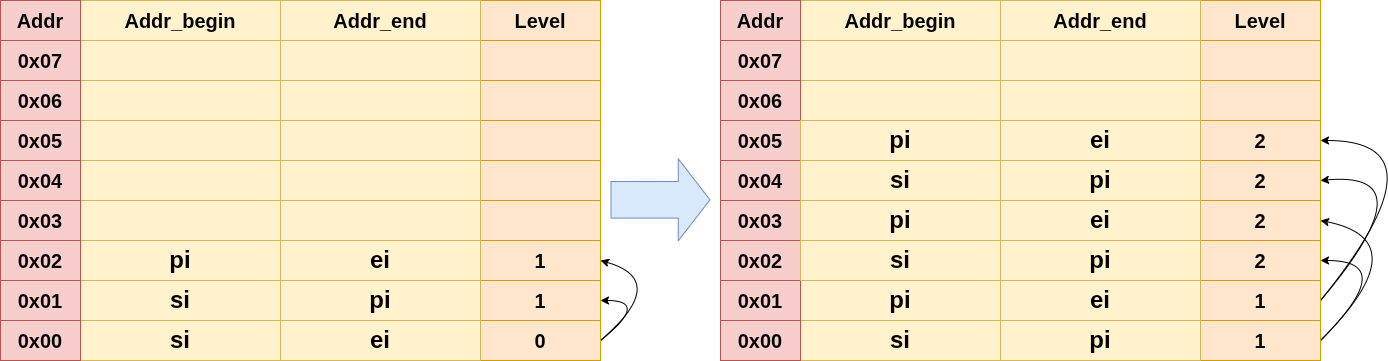
\includegraphics[width=.8\linewidth]{./my-chapters/my-images/SLT/stack_diagram.png}
	\caption{Cấu trúc của bộ lưu trữ stack khi thay thế cho đệ quy.}
\end{figure}

Nhờ đó, giải thuật đệ quy cho phép chia mảng thành từng đoạn $N/2$ được trực quan hóa hơn và dễ dàng kiểm soát hơn về mặt độ rộng, độ sâu của bộ nhớ stack thêm vào. Sau đây là so sánh giữa hai giải thuật:

\begin{table}[H]
	\centering
	{
		\fontsize{11}{10}\selectfont
		\renewcommand{\arraystretch}{1.5}
		\begin{tabular}{@{}p{4cm} p{5.5cm} p{5.5cm}@{}}
			\toprule
			\textbf{Tiêu chí} & \textbf{Recursive (Serial)} & \textbf{Iterative (RTL)} \\
			\midrule
			\textbf{Thời gian (Average Case)} & $O(N \log N)$ & $O(N \log N)$ \\
			\textbf{Thời gian (Worst Case)} & $O(N^2)$ & $O(N^2)$ \\
			\textbf{Không gian (Space)} & $O(M)$ hoặc $O(\log N)$ \newline (System Call Stack) & $O(M)$ hoặc $O(\log N)$ \newline (Heap Memory - \texttt{std::vector}) \\
			\textbf{Chi phí quản lý (Overhead)} & Cao (do khởi tạo stack frame cho mỗi lần gọi hàm). & Thấp (chỉ thao tác \texttt{push/pop} trên vector). \\
			\textbf{Rủi ro bộ nhớ} & Dễ gây \textit{Stack Overflow} khi $N$ lớn hoặc $M$ sâu. & An toàn hơn, giới hạn bởi dung lượng RAM (Heap). \\
			\bottomrule
		\end{tabular}
	}
	\caption{Bảng so sánh độ phức tạp và tài nguyên giữa bộ \texttt{Division\_Recursive} và bộ \texttt{Division\_Iterative}.}
\end{table}

\subsection{Kết quả của thuật toán sau khi viết lại}

\begin{figure}[H]
	\centering
	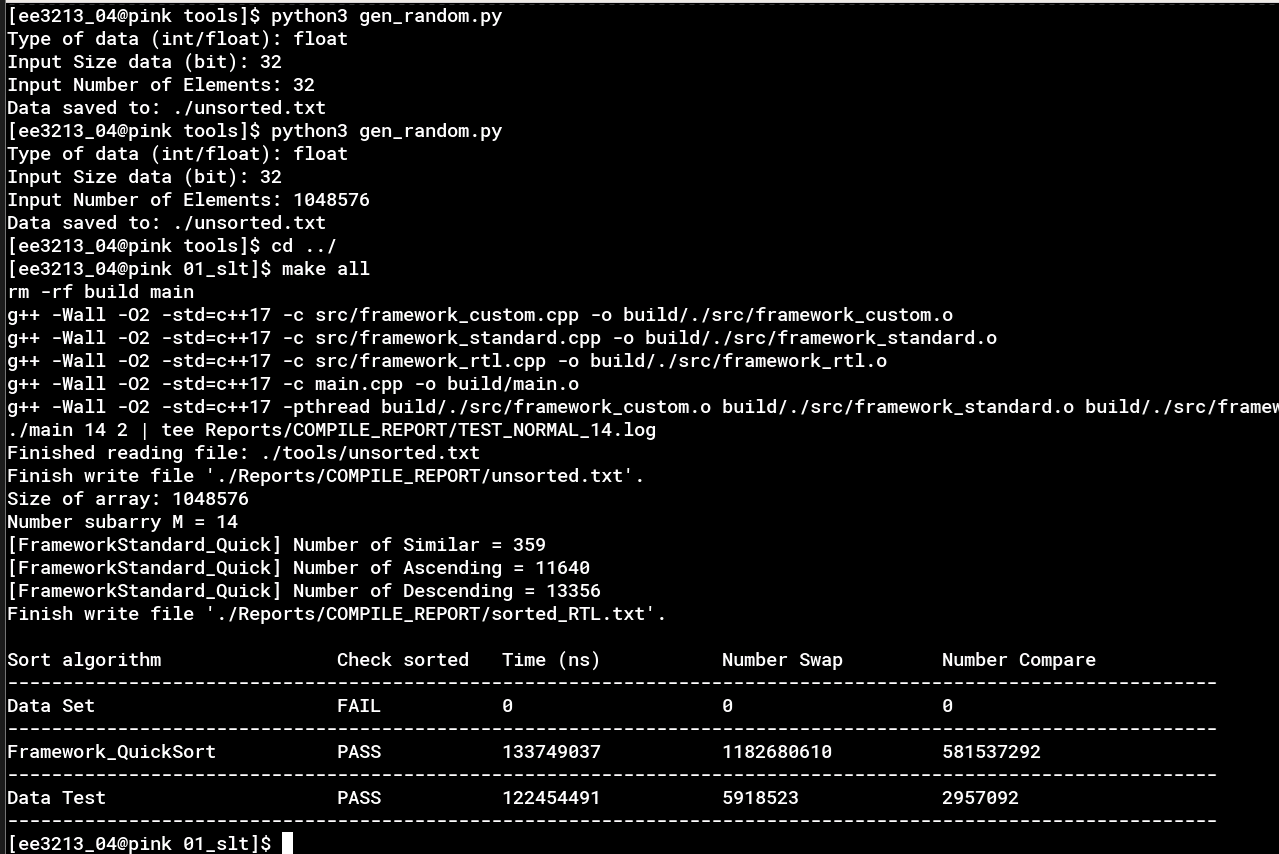
\includegraphics[width=.9\linewidth]{./my-chapters/my-images/SLT/Sort_2_20.png}
	\caption{Kết quả so sánh giữa bộ Framework chuẩn và Framework chỉnh sửa.}
\end{figure}

\begin{figure}[H]
	\centering
	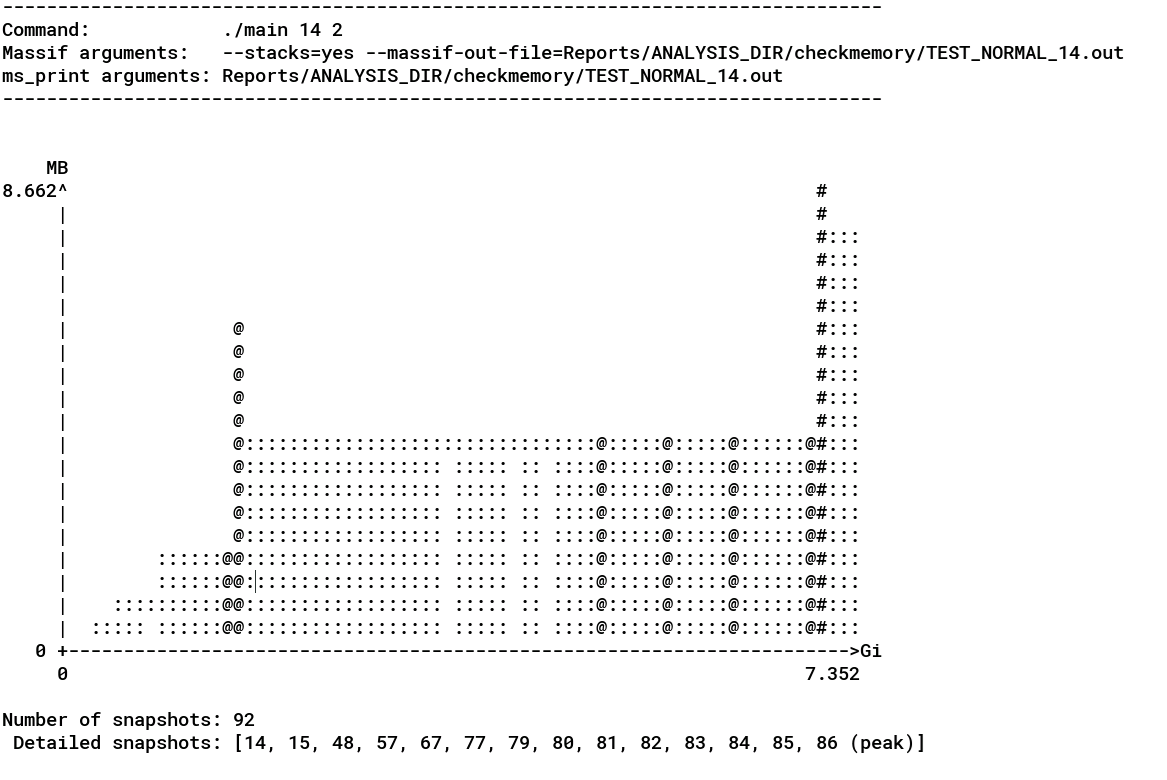
\includegraphics[width=.9\linewidth]{./my-chapters/my-images/SLT/mem_framework_standard_2_20.png}
	\caption{Kết quả của việc sử dụng Memory khi sử dụng Framework chuẩn.}
\end{figure}

\begin{figure}[H]
	\centering
	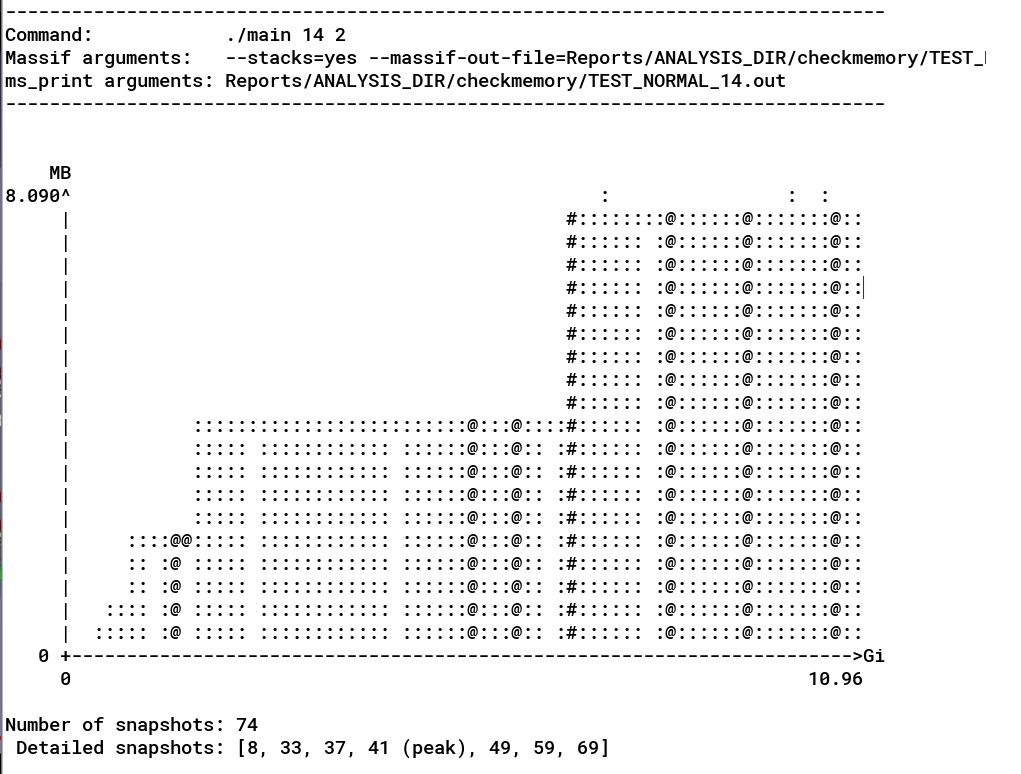
\includegraphics[width=.9\linewidth]{./my-chapters/my-images/SLT/mem_framework_rtl_2_20.png}
	\caption{Kết quả của việc sử dụng Memory khi sử dụng Framework chỉnh sửa.}
\end{figure}

Như vậy, sau khi tối ưu framework thì có số lượng Number Compare và Number Swap ít hơn tương đối so với framework chính thống.